\documentclass{article}

% Packages required by doxygen
\usepackage{calc}
\usepackage{doxygen}
\usepackage[export]{adjustbox} % also loads graphicx
\usepackage{graphicx}
\usepackage[format=hang]{caption}
\usepackage{subcaption}
\usepackage[utf8]{inputenc}
\usepackage{makeidx}
\usepackage{multicol}
\usepackage{multirow}
\PassOptionsToPackage{warn}{textcomp}
\usepackage{textcomp}
\usepackage[nointegrals]{wasysym}
\usepackage[table]{xcolor}
\usepackage{amsmath}

% set up graphicx package
\graphicspath{{./images/}}
\DeclareGraphicsExtensions{.png, .eps}

% definitions for title and footer
\newcommand{\insdate}{\mbox{Fri Feb 5 2016 }}
\newcommand{\institle}{\mbox{Cloth Simulation }}

% Font selection
\usepackage[T1]{fontenc}
\usepackage[scaled=.90]{helvet}
\usepackage{courier}
\usepackage{amssymb}
\usepackage{sectsty}
\renewcommand{\familydefault}{\sfdefault}
\allsectionsfont{%
  \fontseries{bc}\selectfont%
  \color{darkgray}%
}
\renewcommand{\DoxyLabelFont}{%
  \fontseries{bc}\selectfont%
  \color{darkgray}%
}
\newcommand{\+}{\discretionary{\mbox{\scriptsize$\hookleftarrow$}}{}{}}

% Page & text layout
\usepackage{geometry}
\geometry{%
  a4paper,%
  top=2.5cm,%
  bottom=2.5cm,%
  left=2.5cm,%
  right=2.5cm%
}
\tolerance=750
\hfuzz=15pt
\hbadness=750
\setlength{\emergencystretch}{15pt}
\setlength{\parindent}{0cm}
\setlength{\parskip}{0.2cm}
\makeatletter
\renewcommand{\paragraph}{%
  \@startsection{paragraph}{4}{0ex}{-1.0ex}{1.0ex}{%
    \normalfont\normalsize\bfseries\SS@parafont%
  }%
}
\renewcommand{\subparagraph}{%
  \@startsection{subparagraph}{5}{0ex}{-1.0ex}{1.0ex}{%
    \normalfont\normalsize\bfseries\SS@subparafont%
  }%
}
\makeatother

% Headers & footers
\usepackage{fancyhdr}
\pagestyle{fancyplain}
\fancyhead[LE]{\fancyplain{}{\bfseries\thepage}}
\fancyhead[CE]{\fancyplain{}{}}
\fancyhead[RE]{\fancyplain{}{\bfseries\leftmark}}
\fancyhead[LO]{\fancyplain{}{\bfseries\rightmark}}
\fancyhead[CO]{\fancyplain{}{}}
\fancyhead[RO]{\fancyplain{}{\bfseries\thepage}}
\fancyfoot[LE]{\fancyplain{}{}}
\fancyfoot[CE]{\fancyplain{}{}}
\fancyfoot[RE]{\fancyplain{}{\bfseries\scriptsize Final Project for Physically based Simulation WS\,2015/16: \institle, \insdate }}
\fancyfoot[LO]{\fancyplain{}{\bfseries\scriptsize Final Project for Physically based Simulation WS\,2015/16: \institle, \insdate }}
\fancyfoot[CO]{\fancyplain{}{}}
\fancyfoot[RO]{\fancyplain{}{}}
\renewcommand{\footrulewidth}{0.4pt}

\renewcommand{\sectionmark}[1]{%
  \markright{\thesection\ #1}%
}

% Indices & bibliography
\usepackage{natbib}
\usepackage[titles]{tocloft}
\setcounter{tocdepth}{3}
\setcounter{secnumdepth}{5}
\makeindex

% Hyperlinks (required, but should be loaded last)
\usepackage{ifpdf}
\ifpdf
  \usepackage[pdftex,pagebackref=true]{hyperref}
\else
  \usepackage[ps2pdf,pagebackref=true]{hyperref}
\fi
\hypersetup{%
  colorlinks=true,%
  linkcolor=blue,%
  citecolor=blue,%
  unicode%
}

% Custom commands
\newcommand{\clearemptydoublepage}{%
  \newpage{\pagestyle{empty}\cleardoublepage}%
}


%===== C O N T E N T S =====

\begin{document}

% Titlepage & ToC
\hypersetup{pageanchor=false,
             bookmarks=true,
             bookmarksnumbered=true,
             pdfencoding=unicode
            }
\begin{titlepage}
\vspace*{7cm}
\begin{center}%
{\huge Physically Based Simulation }\\
\vspace*{0.3cm}
{\Large Pro-Seminar WS\,2015/16 }\\
\vspace*{1.5cm}
{\Large \institle }\\
\vspace*{1cm}
{\large Elias Zischg, Daly Chea, Gerhard Aigner}\\
\vspace*{0.5cm}
{\small \insdate}\\
\end{center}
\end{titlepage}
\hypersetup{pageanchor=true}

\section{Introduction}
This project is about the simulation of a piece of cloth interacting with rigid bodies.\par

During the simulation, the cloth interacts with its environment i.e. self-collision and cloth-object collision must be regarded. We use collision detection between the cloth object represented as mass spring system and rigid body objects represented as triangle mesh. Self-collision of the cloth object is not considered.\par

The collision response method uses spring penalty forces for the mass points of the cloth object. The rigid objects do not respond to collisions. The equation of motion for the mass spring system is solved by a symplectic euler method.\par

The appearance of the cloth is primarily the response to these conditions. The simulation shows the cloth falling down and covering a sphere object. We use OpenGL to render the scene.
\section{Set-up of the scene}
The modeling of the scene has been done with the 3D-graphics software \textit{blender}. Figure \ref{fig:blender} shows a screen-shot with the model used for the cloth simulation. Once, the wire-frame and the texturing is done, the model is exported as wavefront object. The result is a \textit{.obj}-file and a \textit{.mat}-file. In a post-processing step with the \textit{blender2oGL} \footnote{The \textit{blender2oGL} tool is available from our project repository on GitHub: \url{https://github.com/3eee3/ez-dc-ga}.} tool, also developed during the project, the \textit{.obj}-file is translated to a set of C-source and header files, ready to include into the project. Thus, almost any scene setting is easily included into the cloth simulation program, as long as the target computer can handle the processing effort\footnote{The algorithms to compute the physics simulation and the collision detection are quite CPU-time expensive. Besides that, the computation is forced onto one single core, such that only small scenes will run smooth and seamless.}.
\begin{figure}[h]
	\centering
	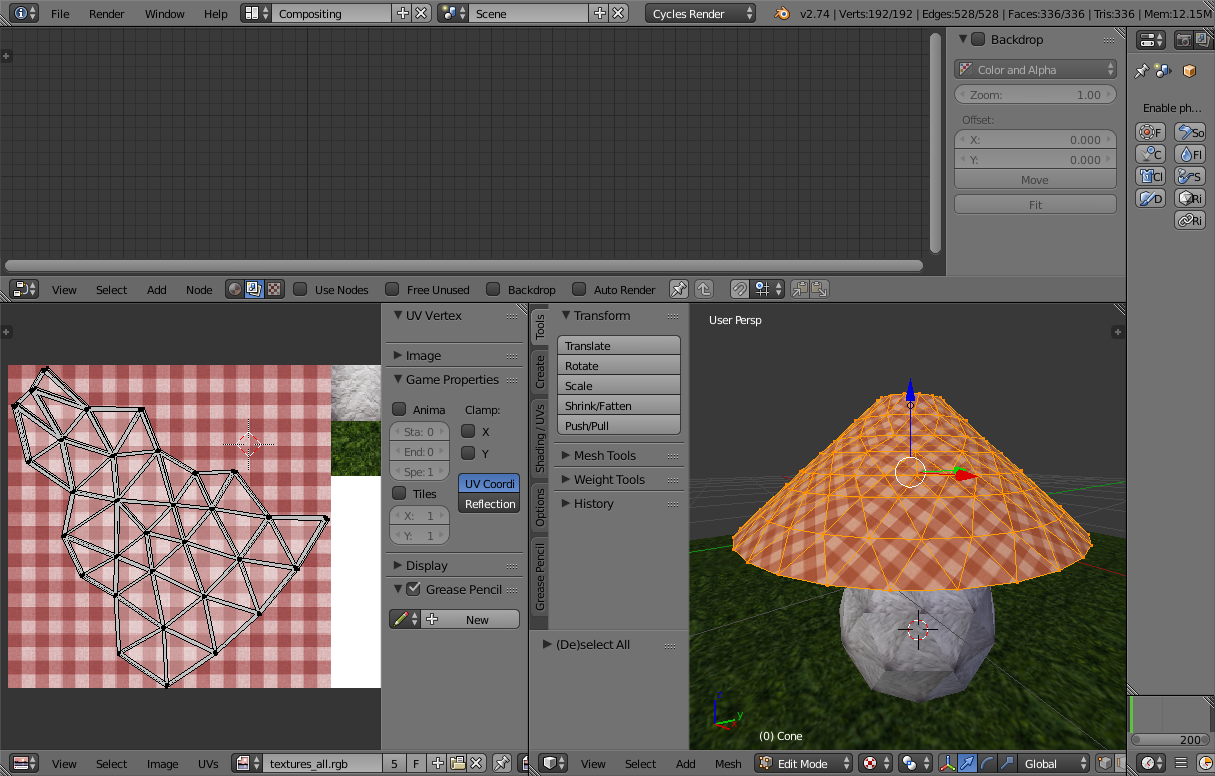
\includegraphics[width=\textwidth]{skirt_sphere_blend}
	\caption{Blender is used to set up a model. Subsequently, the model is exported as wavefront object file and converted to C-files with the \textit{blender2oGL} tool.}
	\label{fig:blender}
\end{figure}

The initial setting shows a skirt above a sphere. The sphere is hovering above the ground. As shown in figure \ref{fig:scene_wrap}, the skirt falls down, on top of the sphere and wraps around it. After the collision with the surface of the sphere, the cloth slips off, driven by the gravity, applied to the not exactly centered cloth. The penalty force of the collision detection algorithm has also an effect which drives the skirt off the sphere. Finally, the skirt falls down to the floor, where it collides with many wrinkles.\par
We decided to implement different scenes for debugging reasons\footnote{During the implementations happened some obstacles which led to non-running code. Because of that, we created a reduced version of the \textit{skirt} program without the connection to the \textit{blender} generated model. It contains a hard-coded grid of masses and springs with two corners fixed on top. It is also available on our project repository.}. So, a second scene with two dice is available by uncommenting the line
\begin{verbatim}
#define _DEBUG_OGL_MODEL
\end{verbatim}
in the file \textit{model\_mapping.cpp}.

\begin{figure}[h]
	\centering
	\begin{subfigure}{0.48\textwidth}
		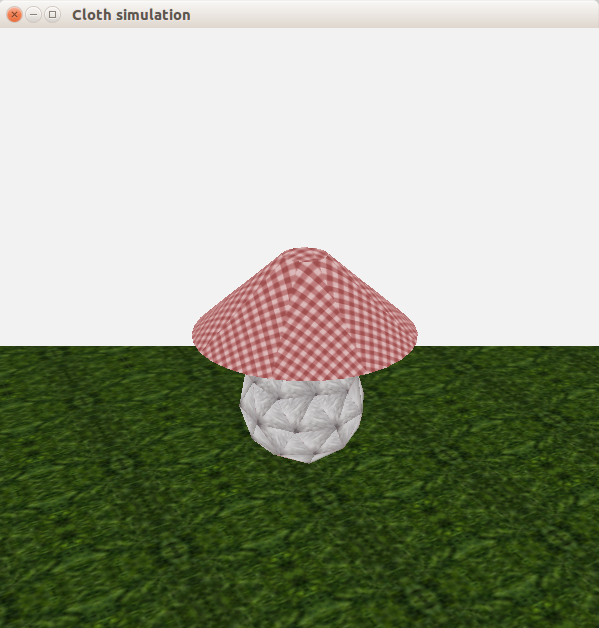
\includegraphics[width=\textwidth]{cloth_sim_initial_scene}
		\subcaption{Initial scene.}
		\label{fig:scene_init}
	\end{subfigure}
	\\
	\begin{subfigure}{0.48\textwidth}
		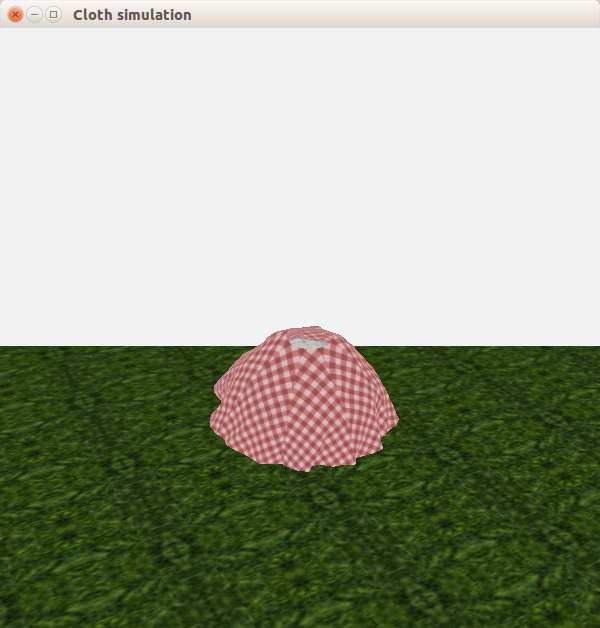
\includegraphics[width=\textwidth]{cloth_sim_wrapped_sphere}
		\subcaption{Sphere wrapped by the cloth.}
		\label{fig:scene_wrap}
	\end{subfigure}
	\quad
	\begin{subfigure}{0.48\textwidth}
		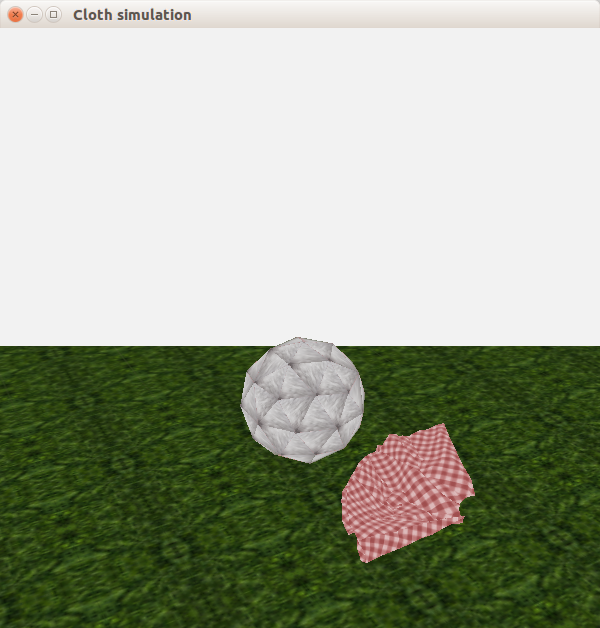
\includegraphics[width=\textwidth]{cloth_sim_skirt_on_floor}
		\subcaption{Finally the skirt falls down to the floor.}
		\label{fig:scene_floor}
	\end{subfigure}
	\caption{The cloth is initially placed above a sphere. It falls down onto the sphere and slips off to the floor.}
	\label{fig:scene}
\end{figure}

\section{Mass Spring System implementation on cloth}
The cloth model is represented by a grid of triangles with a given mass to each point and those triangles are connected by a series of springs.\par

There are three types of spring which are needed to get the characteristics of cloth: 
\begin{itemize}
	\item Structural springs: Handle extension and compression and are connected vertically and horizontally. 
	\item Shear springs: Handle shear stresses and are connected diagonally. 
	\item Bend springs: Handle bending stresses and are connected vertically and horizontally to every other point. 
\end{itemize}

In our cloth simulation, only structural springs and bend springs are used. We use structural springs for all triangles and bend springs for all the springs connected the neighboring triangles. As the two neighboring triangles can always maintain rectangular shapes, there is no need to use the Shear springs on it. See figure \ref{fig:springs} for an example.\par
\begin{figure}[h]
	\centering
	\begin{subfigure}{0.4\textwidth}
		\centering
		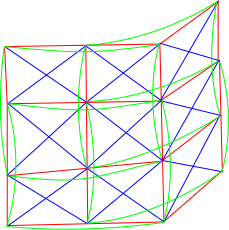
\includegraphics[width=0.6\textwidth]{springs_rectangular}
		\subcaption{Springs applied to a rectangular grid.}
		\label{fig:springs_rect}
	\end{subfigure}
	\quad
	\begin{subfigure}{0.4\textwidth}
		\centering
		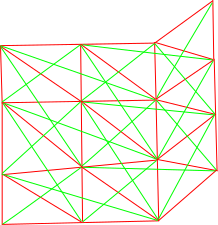
\includegraphics[width=0.6\textwidth]{springs_triangular}
		\subcaption{Springs applied to a triangular grid.}
		\label{fig:springs_triang}
	\end{subfigure}
	\caption{Example of a springs set up for a rectangular and a triangular grid. The structural springs are drawn in red color, bend springs are green colored. The blue shear springs are only applied to a rectangular grid.}
	\label{fig:springs}
\end{figure}

When the simulation is initiated, the rest length of each spring is set to the original length of the springs. The value of the masses and the stiffness of the springs are also set.\par

Once the masses and springs are all set up, and an environmental force, for example gravity, is applied to the points in the model over a specified time step, it produces a resulting acceleration for each point. This acceleration gives rise to a velocity which causes the point to update its position. The new position of each point in turn causes a change in length to each connected spring. The combination of the point and spring forces is integrated with respect to time to provide a new acceleration for each point. Calculating forces and updating positions iteratively provides the motion of the cloth object.

\subsection{Symplectic Euler method for mass-spring simulation}
To simulate the mass-spring network, a Symplectic Euler solver is implemented. Its benefit is a low computation effort in comparison to the other methods used during the pro-seminar. Unfortunately, the drawback is a less accurate result for each simulation step, which leads to integrated numeric errors. In our project accuracy is not important and so, they may be ignored as long the simulation stays stable.

\subsubsection{Algorithm}
For each time-step $h$ do the following steps:\par
For all mass-points compute position $\vec{x}$ at time $t+h$:
\begin{equation}
	\vec{x}(t+h) = \vec{x}(t) + h \cdot \vec{v}(t)
\end{equation}      
Compute forces $\vec{f}$ for all springs with end-points $\vec{x}_1$ and $\vec{x}_2$ at time $t$ considering the already updated values from $\vec{x}(t+h)$:
\begin{align}
	\vec{f}(t)          &= \vec{f}_{int}(t) + \vec{f}_{ext}(t) \text{ with} \\
	\vec{\Delta x}(t)   &= \vec{x}_1(t+h)-\vec{x}_2(t+h) \text{,}\\
	\vec{f}_{int}(t)    &= \frac{\vec{\Delta x}(t)}
	                       {||\vec{\Delta x}(t)||} \cdot k \cdot
	                       \left( l - ||\vec{\Delta x}(t)||\right) 
	                       \text{ and} \\
	\vec{f}_{ext}(t)    &= m \cdot \vec{g} + \vec{F}_P + \vec{f}_{interact}
\end{align}
The parameters $k$ and $l$ are the spring constants and rest lengths of the springs respectively. A ratio of $1 : 8$ for the spring constant $k$ between the bending- and structural springs gave reasonable results.
Interactive forces $\vec{f}_{interact}$ may be generated by any input devices like keyboard or mouse. Actually no interactions are implemented.
\par
Compute acceleration $\vec{a}$ for each point with mass $m$ at time $t$:
\begin{equation}
	\vec{a}(t) = \frac{1}{m} \cdot (\vec{f}(t) - \gamma \cdot \vec{v}(t))
\end{equation}
The damping parameter $\gamma$ is used to simulate friction and air pressure.
Finally, update the velocity $\vec{v}$ of each point at time $t+h$:
\begin{equation}
	\vec{v}(t+h) = \vec{v}(t) + h \cdot \vec{a}(t)
\end{equation}

\section{Collision}
For the project we used collision detection between the cloth object represented as mass spring system and rigid body objects represented as triangle mesh. 

\subsection{Collision detection}
During collision detection every mass point of the cloth is compared with every triangle of the rigid object. If the point lies within an $\varepsilon$-area of the triangle the collision functions returns true, otherwise false. The comparison between a single Point $P$ and a triangle with points $A$, $B$ and $C$ is explained below.\par

At first the triangle normal $n$ and the distance d of the Point P to the triangle plane is computed:
\begin{align}
	n &= (B-A) \times (C-A)\\
	d &= n \cdot P - n \cdot A
\end{align}
If the absolute value of the distance $d$ is greater than  $\varepsilon$ the point does not collide with the triangle.
Otherwise, further checks are necessary. The point $P$ is projected on the plane of the triangle with points $A$, $B$ and $C$ and normal $n$.
\begin{equation}
	P' = P - (n \cdot (P - A)/(n \cdot n))n
\end{equation}
The projected point $P'$ can then be expressed in barycentric coordinates u,v:
\begin{equation}
	P' = A + u(B - A) + v(C - A) = (1 - u - v)A + uB + vC
\end{equation}
The point $P'$ lies in the triangle area if $u\geq 0$ and $v\geq 0$ and $u+v \leq 1$.

\subsection{Collision response}
The implemented collision response method uses spring penalty forces  for the mass points of the cloth object. The collision detection function returns the distance $d$ of the point $P$ to the colliding triangle $T$. The normal $n$ of the colliding triangle is returned as well. The distance  $d$ can be negative or positive depending on which side of the triangle plane the point is located.  In both cases the penalty force $F_P$ is computed as
\begin{equation}
	F_P = k_{rep} \cdot (-1) \cdot (d - \varepsilon) \cdot n
\end{equation}
where $ k_{rep}$ is the repulsive spring constant used for the penalty force and  $\varepsilon$ is the distance from the triangle in which a collision can occur.


\end{document}
